\documentclass[UTF8]{ctexart}

%固定图片位置
\usepackage{float}

%插入超链接
\usepackage{url}

\usepackage{tikz,mathpazo}
\usetikzlibrary{shapes.geometric, arrows}
\usetikzlibrary{calc}


\usepackage{listings}
%插入代码的配置
\definecolor{CPPLight}  {HTML} {686868}
\definecolor{CPPSteel}  {HTML} {888888}
\definecolor{CPPDark}   {HTML} {262626}
\definecolor{CPPBlue}   {HTML} {4172A3}
\definecolor{CPPGreen}  {HTML} {487818}
\definecolor{CPPBrown}  {HTML} {A07040}
\definecolor{CPPRed}    {HTML} {AD4D3A}
\definecolor{CPPViolet} {HTML} {7040A0}
\definecolor{CPPGray}  {HTML} {B8B8B8}
\lstset{
	language=Python,                                     % 设置语言
    columns=fixed,    
    breaklines = true,   
    basicstyle=\small ,
    numbers=left,                                        % 在左侧显示行号
    %frame=none,                                          % 不显示背景边框
    backgroundcolor=\color[RGB]{245,245,244},            % 设定背景颜色
    keywordstyle=\color[RGB]{40,40,255},                 % 设定关键字颜色
    numberstyle=\tiny\color{darkgray},           % 设定行号格式
    %commentstyle=\it\color[RGB]{0,96,96},                % 设置代码注释的格式
    stringstyle=\rmfamily\slshape\color[RGB]{128,0,0},   % 设置字符串格式
    showstringspaces=false,                              % 不显示字符串中的空格                           
    %morekeywords={True,alignas,continute,friend,register,true,alignof,decltype,goto,
    %reinterpret_cast,try,asm,defult,if,return,typedef,auto,delete,inline,short,
    %typeid,bool,do,int,signed,typename,break,double,long,sizeof,union,case,
    %dynamic_cast,mutable,static,unsigned,catch,else,namespace,static_assert,using,
    %char,enum,new,static_cast,virtual,char16_t,char32_t,explict,noexcept,struct,
    %void,export,nullptr,switch,volatile,class,extern,operator,template,wchar_t,
    %const,false,private,this,while,constexpr,float,protected,thread_local,
    %const_cast,for,public,throw,std,rand},
    emph={access,and,break,class,continue,def,del,elif ,else,%
	except,exec,finally,for,from,global,if,import,in,i s,%
	lambda,not,or,pass,print,raise,return,try,while},
    emphstyle=\color{CPPViolet}, 
    emph={[2]True, False, None, self},
	emphstyle=[2]\color{green},
	emph={[3]from, import, as},
	emphstyle=[3]\color{blue},
	upquote=true,
	morecomment=[s]{"""}{"""},
	commentstyle=\color{orange}\slshape,
	emph={[4]1, 2, 3, 4, 5, 6, 7, 8, 9, 0},
	emphstyle=[4]\color{red},
	emph={[5]numpy, np, plt},
	emphstyle=[5]\color{red},
	literate=*{:}{{\textcolor{blue}:}}{1}%
	{=}{{\textcolor{blue}=}}{1}%
	{-}{{\textcolor{blue}-}}{1}%
	{+}{{\textcolor{blue}+}}{1}%
	{*}{{\textcolor{blue}*}}{1}%
	{!}{{\textcolor{blue}!}}{1}%
	{(}{{\textcolor{blue}(}}{1}%
	{)}{{\textcolor{blue})}}{1}%
	{[}{{\textcolor{blue}[}}{1}%
	{]}{{\textcolor{blue}]}}{1}%
	{<}{{\textcolor{blue}<}}{1}%
	{>}{{\textcolor{blue}>}}{1},%
	framexleftmargin=0.1mm, framextopmargin=0.1mm, frame=shadowbox, rulesepcolor=\color{black},
}



\usepackage{geometry}
\geometry{left=2cm, right=2cm, top=1.2cm, bottom=1.2cm}

%得到引用的标题内容
\usepackage{nameref} 

%添加首行缩进,两个字符
\usepackage{indentfirst}
\setlength{\parindent}{2em}

%多行公式一个编号
\usepackage{amsmath}

%文献引用,标准类型为plain
%\usepackage[hyperref=true,backend=biber,sorting=none,backref=true]{biblatex}
%\addbibresource{ref.bib}
\bibliographystyle{plain}
\usepackage{cite}

\pagestyle{plain}

%跨页表格
\usepackage{multirow}
\usepackage{longtable,booktabs}
\usepackage{supertabular}
\usepackage{makecell}

%调整itemize等的间距
\usepackage{enumitem}


\usepackage{graphicx}
\usepackage{subfigure}

%超链接
\usepackage[linkcolor=yellow,citecolor=red,backref=page,hyperfootnotes=true]{hyperref}
\hypersetup{
bookmarks=true,
colorlinks=true,
linkcolor=black
}
\usepackage{tabularx} %This package must be placed after package {hyperref}, otherwise footnote marks are NOT treated as hyperlinks.


%引入了一些改进的数学环境,如align
\usepackage{amsmath}

\title{数字图像实验报告一}
\author{姓名:鲁国锐 \protect\newline
\and 学号:17020021031 \\
\and 专业:电子信息科学与技术}


\begin{document}
	\maketitle
	\renewcommand{\contentsname}{目录}
	\renewcommand{\listfigurename}{插图目录}
	\renewcommand{\listtablename}{表格目录}
	\renewcommand{\refname}{参考文献}
	\renewcommand{\abstractname}{摘要}
	\renewcommand{\indexname}{索引}
	\renewcommand{\tablename}{表}
	\renewcommand{\figurename}{图}
	\tableofcontents
	\newpage
	
	\hypersetup{
	bookmarks=true,
	colorlinks=true,
	linkcolor=red,
	urlcolor=blue
	}
	\section{问题分析}
	\subsection{题目描述}
	\indent 本次实验任务分为两部分。第一个部分是熟练$MATLAB$或$Python$的操作,将图像读取后改变大小,转换为灰度图,并保存为$gif$格式;第二部分是用一副小图像拼成另一幅图,做成一副主题图像。

%     \subsection{输入}
%     \indent 第一行为两个整数$n$,$m$,分别为小镇的个数以及接下来小于$20km$的小镇对的数目。 接下来的$m$行,每行$2$个整数,表示两个小镇的距离小于$20km$(编号从$1$开始)。
%     
%     \subsection{输出}
%     \indent 如果能够满足要求,输出$1$,否则输出$-1$。

	\subsection{问题分析}\label{analysis}
	\indent 第一部分的任务不复杂,主要是熟悉几个基本函数的用法,在此不多做介绍。
	
	\indent 沿着这条思路,又可以把该问题分为三个子问题:
	\begin{enumerate}[leftmargin=50pt]
	\item 分别确定纸带正常区域及缺损区域的像素值范围;\label{problem1}
	\item 判断像素值在缺损范围的各个像素点是否连成一个区域,且该区域大到无法忽视的地步;\label{problem2}
	\item 排除其它因素的干扰(背景、阴影等)。\label{problem3}
	\end{enumerate}
	
	\indent 我们将在下一节中对这三个子问题分别进行讨论。
	
	

	
	\section{解决方案}
		\subsection{确定像素值范围}
		
			\indent 针对\ref{analysis}节中的问题\ref{problem1},可以直接通过实验的方法来确定。
%			
%			\begin{figure}[H]
%				\centering 
%				\includegraphics[scale=0.05]{paper0.jpg} 
%				\caption{实验样例$1$} 
%				\label{paper0}
%			\end{figure}
%			
%			\indent 图\ref{paper0}是一张普通卫生纸被撕开一块后,放在黑色背景下拍得的一张照片。但由于该图像分辨率较高,数据量大,不利于观察,所以将其裁剪后得到图\ref{paper3}。
%		
%			\begin{figure}[H]
%				\centering 
%				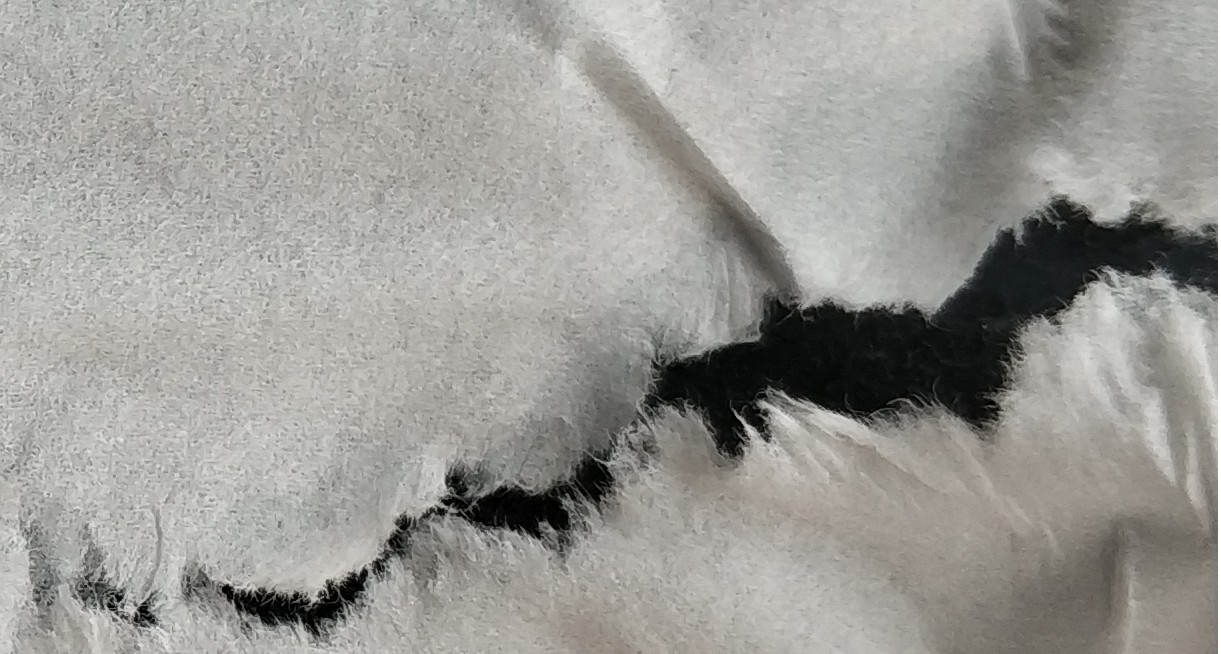
\includegraphics[scale=0.3]{paper3.jpg} 
%				\caption{实验样例$2$(从样例$1$中截取得到)} 
%				\label{paper3}
%			\end{figure}
%			
%			\indent 用$MATLAB$读取图\ref{paper3}并输出其像素值,可以明显发现正常区域的像素值基本大于$150$,而破损处的像素值集中在$50$以下。
%			
%			\indent 同理,将墨水滴于纸上来模拟污损或斑点,得到图\ref{paper5}和图\ref{paper6}。
%			
%			\begin{figure}[H]
%				\centering 
%				\includegraphics[scale=0.05]{paper5.jpg} 
%				\caption{实验样例$3$} 
%				\label{paper5}
%			\end{figure}
%		
%			\begin{figure}[H]
%				\centering 
%				
\includegraphics[scale=1]{paper6.jpg} 
%				\caption{实验样例$4$(从样例$3$中截取得到)} 
%				\label{paper6}
%			\end{figure}
		
			\indent 采用相同的方法可以得到污损区域的像素值范围。污损与破损像素值的变化有所不同:破损区域像素值的跳变明显;而污损区域的像素值由外到里变化相对平缓(由图\ref{paper6}可以看出)。总体而言,污损区域的像素值集中在$120$以下,但后续实验的结果(见第\ref{results}节)表明,将阈值设为$80$更为合适。
		\subsection{判断非正常像素点是否连成一个足够大的区域}
			
			\indent 针对\ref{analysis}节的问题\ref{problem2},我们采用“深度优先搜索($DFS$)”的方法。
			
			\subsubsection{算法描述}\label{algorithm}
			
				\indent 对于一张已得到的图像,从头开始遍历每一个像素,每当发现当前像素的取值不在正常范围内时,就开始进行深度优先搜索。搜索从该点开始,向其上下左右及主副对角线共$8$个方向进行递归查找。
				
				\indent 每次递归时,首先判断该位置是否在图像范围内,其次判断该位置的像素值是否在非正常范围内。只有当上述两个条件均满足时,才继续进行递归。同时为了保证搜索不重复,需要将该点的像素值置为$255$。
				
			\subsubsection{采用面向对象的方法降低时间复杂度}
			
				\indent $MATLAB$与$C$语言或$C++$相比,一个重要的不同之处是$MATLAB$无法进行引用或指针的传递。也就是说我们无法在递归的过程中对原图像矩阵做标记,每次递归时都必须把整个矩阵复制一遍,这样增加了很多不必要的开销。
				
				\indent 针对这种情况,我们采用面向对象的方法,将图像矩阵与\ref{algorithm}节中涉及的函数封装成一个类,这样就可把图像矩阵作为全局变量,从而避免“值传递”产生的额外开销。同时还可以把与之相关的其它特征参数也作为成员变量,如维度、阈值等,这样可以避免反复调用$size$等函数,也增加了程序的可移植性。
				
			\subsubsection{采用剪枝的方法降低时间复杂度}
				
				\indent 由于本题的要求仅仅是检测纸带是否有缺陷,所以其实无需把不合规的像素点全都遍历一遍。为此可以再增加两个成员变量:一个用于计数在当前缺陷区域中已经访问过的连续非正常像素点的数量;另一个是针对该数量的阈值,由人事先设定好。当发现连续非正常像素点的数量已经超过了阈值时,就可以判定该纸带是有缺陷的,直接结束整个程序。这样一方面可以大大降低程序运行的时间,减少图片大小及其分辨率对程序运行时间的影响;同时还可以避免当缺陷区域过大时递归层数过多,导致内存溢出的问题。
				
		\subsection{排除其它因素的干扰}
			
			\indent 针对\ref{analysis}节中的问题\ref{problem3},本文主要考虑两大干扰因素:
			\begin{enumerate}[leftmargin=50pt]
				\item 背景因素:该问题可以在图像的获取阶段解决,只要保证在得到图像时纸带刚好充满整个画面即可;
				\item 阴影因素:该问题可通过调整阈值解决——阴影部分的像素值大小要比缺陷处大。
			\end{enumerate}
	\section{算法设计}
%
%		\begin{figure}[H]
%			\centering 
%			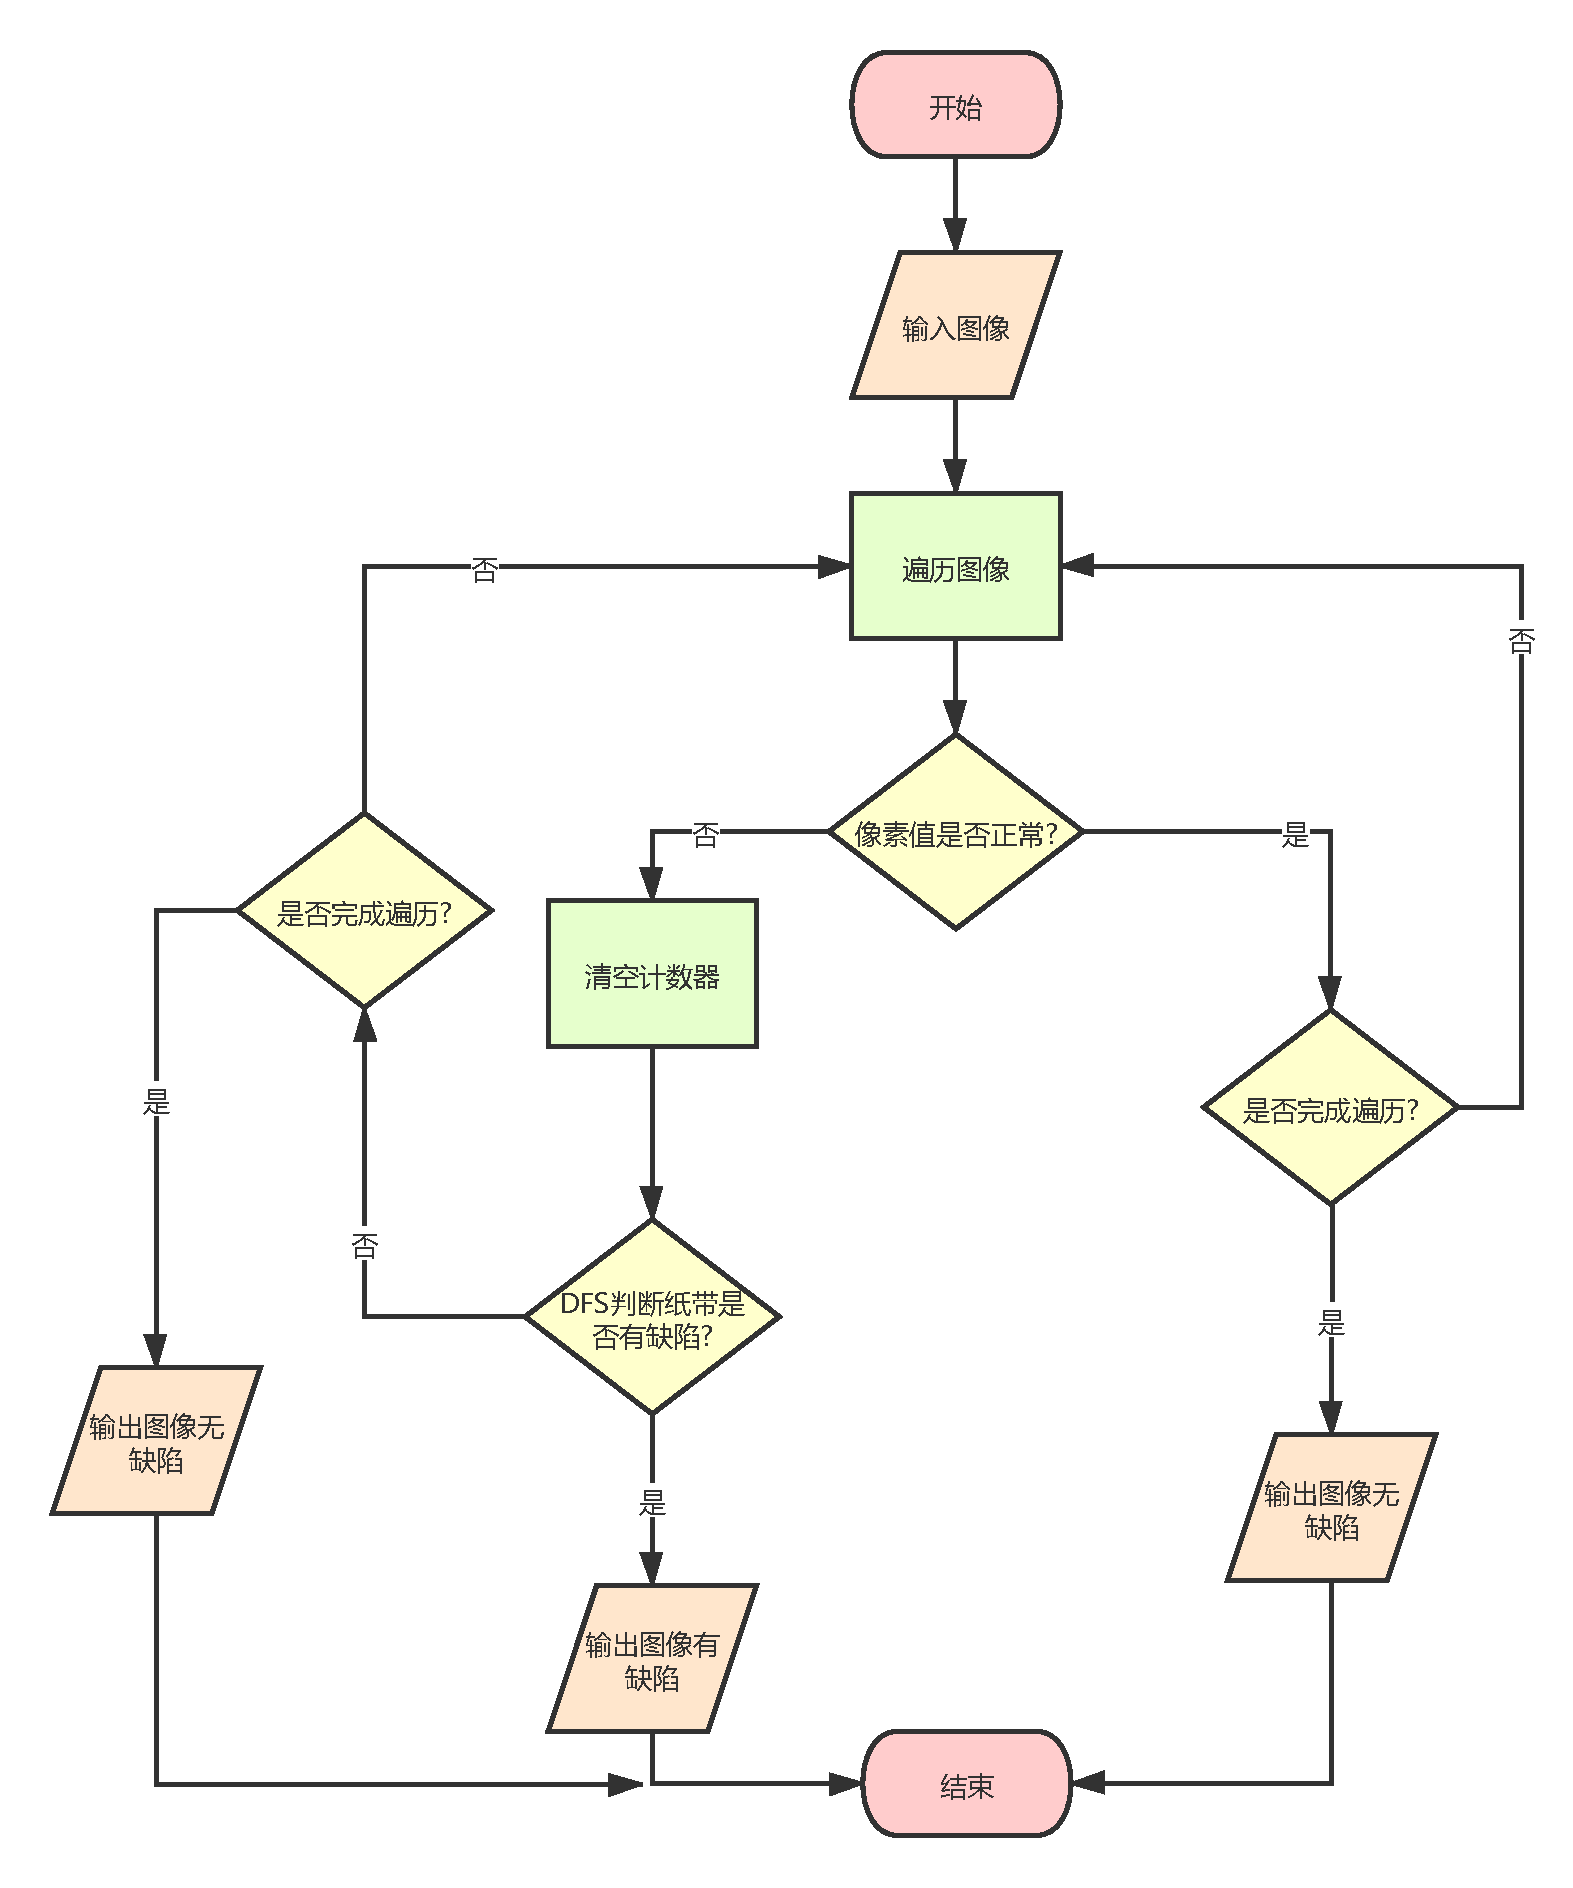
\includegraphics[scale=0.7]{main.pdf} 
%			\caption{$main$函数流程图} 
%			\label{main}
%		\end{figure}




	\section{编程实现\protect \footnotemark[1]}
	\footnotetext[1]{代码也可从该网址获取:\url{https://github.com/chenfeng123456/CourseInOUC/blob/master/Digital_Image_Processing/codes/img_detection.m}}

	\begin{lstlisting}[language=python,caption={boradcast.cpp},label={broadcast.cpp}]
import numpy as np
import matplotlib.pyplot as plt
from PIL import Image
import imageio

# 注意这里dim[0]指的是列数,dim[1]指的是行数
# 转成np数组后会有一次转置
dim = (8, 8)

smile = Image.open('smile.jpg')
smile = smile.resize( dim ).convert('RGB')
smile = np.array(smile)

#########################################################################
# 对笑脸做尺度变换,使其像素值在0~255之间
#########################################################################
min_smile = [256, 256, 256]
max_smile = [0, 0, 0]

for i in range( len(smile) ):
    for j in range( len(smile[i]) ):
        for c in range(0, 3):
            if smile[i][j][c] < min_smile[c]:
                min_smile[c] = smile[i][j][c]
            elif smile[i][j][c] > max_smile[c]:
                max_smile[c] = smile[i][j][c]

for i in range( len(smile) ):
    for j in range( len(smile[i]) ):
        for c in range(0, 3):
            smile[i][j][c] = 255 / (max_smile[c] - min_smile[c]) * (smile[i][j][c] - min_smile[c])
#########################################################################



elephant = Image.open('01.jpg')
print(elephant.size)
elephant = elephant.resize( (elephant.size[0]//dim[0]*dim[0], elephant.size[1]//dim[1]*dim[1]) )
print(elephant.size)
elephant = elephant.convert('RGB')
elephant = np.array(elephant)


for i in range( len(elephant) ):
    for j in range( len(elephant[i]) ):
        for c in range(0, 3):
            temp = float(elephant[i][j][c])
            temp = temp * smile[ i % dim[1] ][ j % dim[0] ][c] / 255.0
            elephant[i][j][c] = temp

plt.figure('elephant')
plt.imshow(elephant)
plt.show()

im = Image.fromarray(elephant)
print(im.size)
im.save('res.jpg')
	\end{lstlisting}

	\section{结果展示与分析}\label{results}
		\subsection{结果展示}\label{show}
%	
%			\begin{figure}[H]
%				\centering 
%				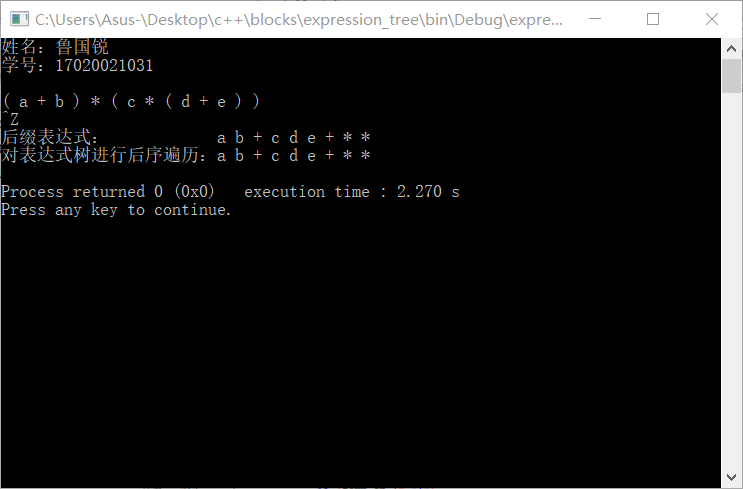
\includegraphics[scale=0.3]{res1.png} 
%				\caption{结果1} 
%				\label{res1}
%			\end{figure}
%		
%			\begin{figure}[H]
%				\centering 
%				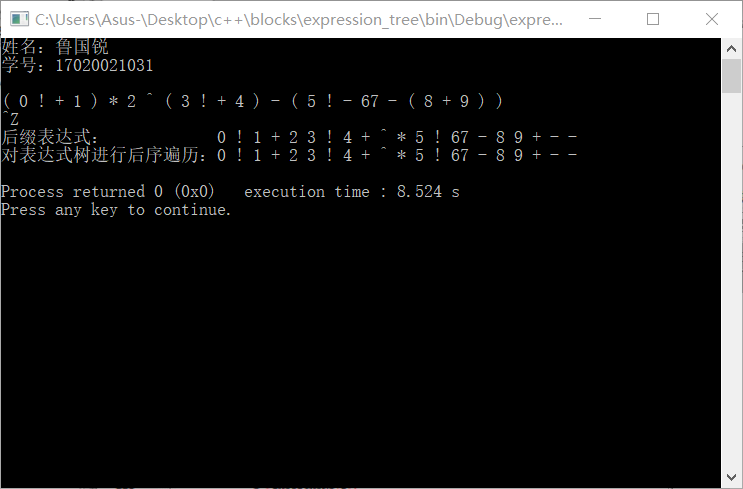
\includegraphics[scale=0.3]{res2.png} 
%				\caption{结果2} 
%				\label{res2}
%			\end{figure}
%		
%			\begin{figure}[H]
%				\centering 
%				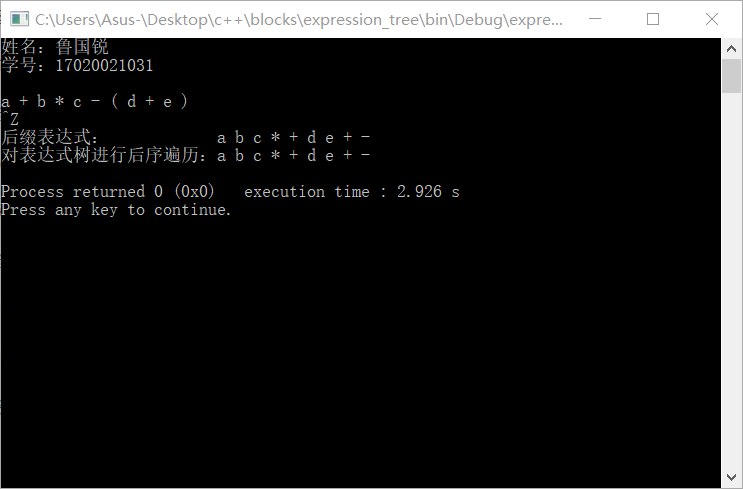
\includegraphics[scale=0.4]{res3.png} 
%				\caption{结果3} 
%				\label{res3}
%			\end{figure}
%		
%			\begin{figure}[H]
%				\centering 
%				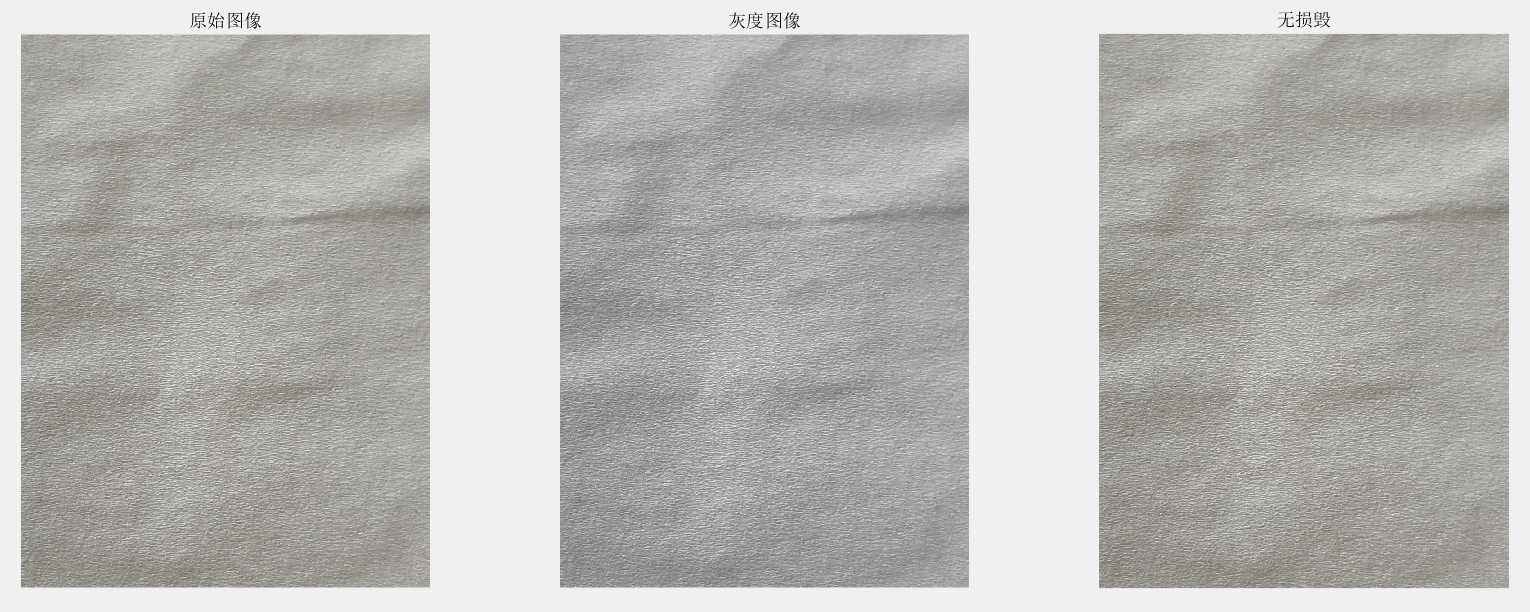
\includegraphics[scale=0.4]{res4.png} 
%				\caption{结果4} 
%				\label{res4}
%			\end{figure}
%		
%			\begin{figure}[H]
%				\centering 
%				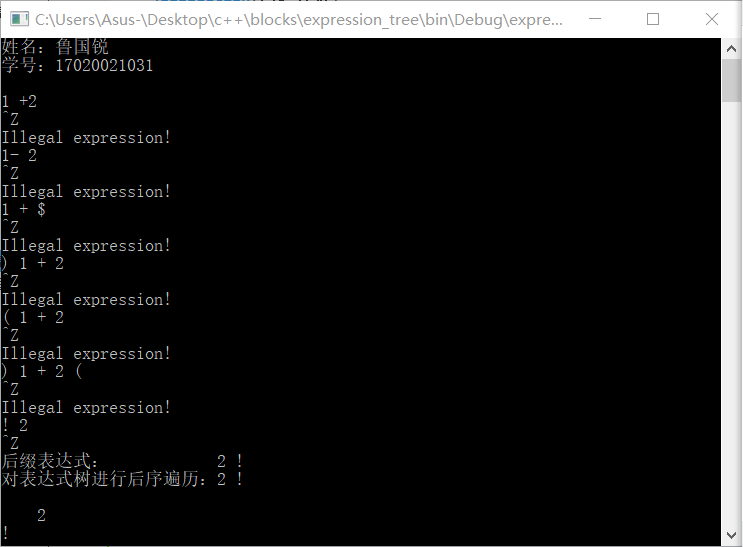
\includegraphics[scale=0.4]{res5.png} 
%				\caption{结果5} 
%				\label{res5}
%			\end{figure}
%		
%			\begin{figure}[H]
%				\centering 
%				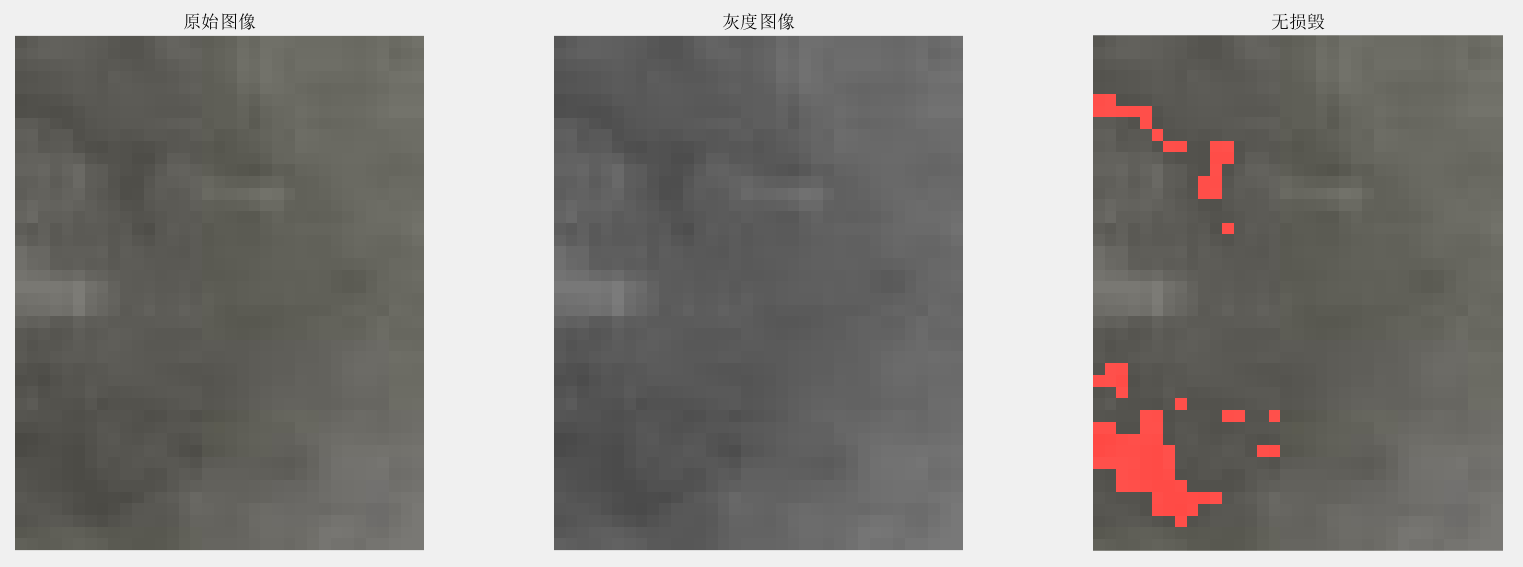
\includegraphics[scale=0.4]{res6.png} 
%				\caption{结果6(截取自结果5的阴影部分)} 
%				\label{res6}
%			\end{figure}
%	
		\subsection{结果分析}
			\indent 从\ref{show}小节中的结果可以看出,在纸带充满整个图像的情况下,该方案可以有效地检测出纸带是否损毁。尤其是从图\ref{res6}可以看出,在像素阈值为$80$的情况下,虽然会有部分阴影处被认为是损毁,但不会有连续大面积的误判,证明通过调节阈值大小可以较为有效地排除阴影部分对于检测的影响。
	\section{总结体会}
		\indent 本次报告所提出的方案在白纸黑背景的情况下能达到较好的效果,但在其它情况下效果如何,受实验条件制约,未能进一步验证。另外,在提出方案的最初,其实是希望能在检测纸带是否有损毁的同时,还能用红色标记出损毁区域。但在本次报告所提的方案中,标出所有损毁区域意味着要用递归遍历所有相关像素点,对于损毁区域较大的样例,会导致内存溢出,故舍弃了该功能。

%\bibliography{ref.bib}
\end{document}